%%%%%%%%%%%%%%%%%%%%%%%%%%%%%%%%%%%%%%%%%%%%%%%%%%%%%%%%%%%
%                                                         %
%       This is documentation for the IPK project.        %
%                                                         %
%%%%%%%%%%%%%%%%%%%%%%%%%%%%%%%%%%%%%%%%%%%%%%%%%%%%%%%%%%%


%------------------------------------------------%
%	    CONFIGURATION + IMPORTED PACKAGES        %
%------------------------------------------------%
\documentclass[10pt,a4paper,titlepage]{article}
\usepackage[english]{babel}
\usepackage[utf8]{inputenc}
\usepackage[margin=100pt]{geometry}


\usepackage{graphicx}   % Import pictures
\usepackage{ragged2e}   % fullfill paragraphs
%\usepackage{multicol}
%\usepackage{lscape}
\usepackage{xcolor}
%\usepackage{listings}
\usepackage{courier}
\usepackage{caption}

\usepackage[backend=biber]{biblatex}
\addbibresource{dokumentace.bib}



\begin{document}
%-----------------------------------------%
%	            TITLE PAGE                %
%-----------------------------------------%
\begin{titlepage}

\begin{center}
% Headings
\textsc{\LARGE Brno University of technology}\\[0.5cm]
\textsc{\large Faculty of Information Technology}\\[8cm]

% Title - lines
{ \huge \bfseries IPK project 2}\\[0.3cm]
{ \Large \bfseries documentation}\\[0.5cm]
{ \bfseries Martin Benes}\\

\end{center}

\end{titlepage}
\newpage

%-----------------------------------------%
%	              DOCUMENT                  %
%-----------------------------------------%

\pagenumbering{gobble}

The task of the project was to gather informations about DHCP protocol and afterwards write a program in C,
that performs a DHCP starvation attack.

\section*{DHCP}
DHCP is an abbreviation of dynamic host configuration protocol. According to Wikipedia, {\it DHCP is a network management protocol used on TCP/IP networks
whereby a DHCP server dynamically assigns an IP address and other network configuration parameters to each device on a network so they can communicate
with other IP networks. } \cite{DHCPwikipedia}

\begin{figure}
    \centering
    \includegraphics[width=0.35\textwidth]{dhcpcomm.png}
    \caption{ DHCP communication. \cite{DHCPcomm}}
    \label{fig:triangle}
\end{figure}

\printbibliography

\end{document}